\documentclass[tikz]{standalone}
%\usetikzlibrary{calc}
\begin{document}
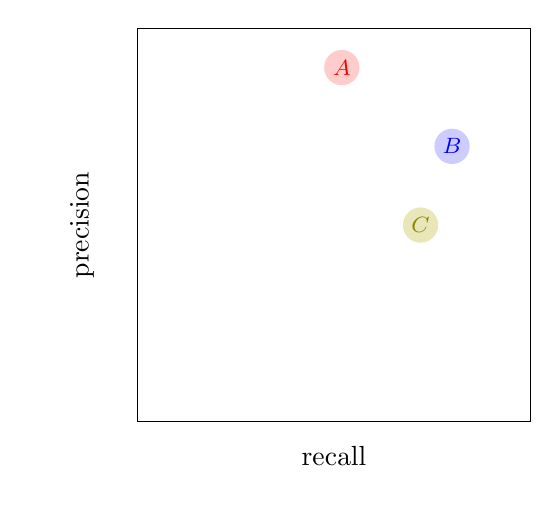
\begin{tikzpicture}[every node/.style={circle, inner sep=0pt}]
\coordinate (SW) at (0,0);
\coordinate (NW) at (0,5);
\coordinate (SE) at (5,0);
\coordinate (NE) at (5,5);

\draw (SW) -- (NW) -- (NE) -- (SE) -- (SW);
\path (SW) -- node[rotate=90, anchor=south] {precision} (NW);
\path (SW) -- node[anchor=north] {recall} (SE);

\coordinate (A1) at (2.6, 4.5);
\coordinate (B1) at (2.1, 4.5);
\coordinate (C1) at (1.3, 4.5);

\coordinate (A2) at (3.5, 3.5);
\coordinate (B2) at (4.0, 3.5);
\coordinate (C2) at (2.75, 3.5);

\coordinate (A3) at (4.05, 2.5);
\coordinate (B3) at (4.70, 2.5);
\coordinate (C3) at (3.6, 2.5);



\footnotesize
\begin{scope}[every node/.style={circle, inner sep=0pt, minimum size=1.5em, red, fill=red!20!white}]
\node at (A1) {\(A\)};
\end{scope}

\begin{scope}[every node/.style={circle, inner sep=0pt, minimum size=1.5em, blue, fill=blue!20!white}]
\node at (B2) {\(B\)};
\end{scope}

\begin{scope}[every node/.style={circle, inner sep=0pt, minimum size=1.5em, olive, fill=olive!20!white}]
\node at (C3) {\(C\)};
\end{scope}

\end{tikzpicture}
\end{document}
